\chapter{Introduction}
\label{sec:intro}
\chaptermark{Introduction}

\begin{center}
\begin{footnotesize}
{ \it{``It has long been an axiom of mine that the little things are infinitely the most important."}}\\
``The Memoirs of Sherlock Holmes", Arthur Conan Doyle\\
\end{footnotesize}
\end{center}

\section{Theoretical Motivation}
\label{sec:introduction}

In some sense, a discovery seemed inevitable. Near Geneva, beneath the foot of the Jura Mountains, the Large Hadron Collider (LHC) has been accelerating protons at higher energies than any collider to date, continuing the fruitful lineage of technological advancement and scientific discovery from earlier particle accelerators. On July 4, 2012, in a joint announcement from CMS and ATLAS, the organizations of the two respective general purpose detectors at the LHC, it was announced that a Higgs-like boson\footnote{Although it is now considered ``a Higgs boson", contemporarily it was deemed ``a Higgs-like boson" until further study could be done.} was observed which opened a new window to probe the foundations of the universe. The genesis of this announcement can be traced to ancient Greece and India with the origins of atomism - the postulate that there exist fundamental, unbreakable constituents that make up all matter - through the discovery of quantum mechanics to today. The Standard Model (SM) is the model proffered by particle physicists for explaining the underpinnings of matter in our universe. This discovery appears to be the observation of the last remaining piece of this model.

Conceived in the 1970s, the SM has been one of the most successful scientific models\footnote{The only possible usurper is special relativity which underlies some of the mathematics of the SM.} ever. Precision tests have repeatedly agreed with SM predictions and fundamental particles which were not observed at the time of conception have since been discovered. The Standard Model's particles and their interactions, along with how they act in the aggregate, can explain nearly all phenomena across any size or time frame in our universe. But, as we will see in Sec.~\ref{sec:SMpreLHC}, there still remain large unanswered questions which we may hope to probe by looking in detail at this new boson.

\subsection{Our Cast of Characters: Fundamental Particles}
\label{sec:FundParticles}

Broadly, the Standard Model consists of a series of point particles with only a few basic characteristics: spin, charge, and mass.

Spin can be thought of as the intrinsic angular momentum of a particle. It can only take integer or half-integer values, which is used to classify particles into two categories: \textit{Bosons} (integer spin) and \textit{Fermions} (half-integer spin). This classification isn't arbitrary; the spin determines the general role of that particle. Fermions obey Fermi-Dirac statistics and therefore cannot occupy identical energy states. These become the building blocks of all observed material in the universe. Bosons instead obey Bose-Einstein statistics -- they are permitted to occupy identical energy states -- and make up the force carriers. If fermions are the pieces, bosons are the glue that binds them.

These particles can interact through any of the four observed forces: Electromagnetism, the Weak and Strong forces, and Gravity. Gravity is a bit problematic and not integrated into the Standard Model (see Sec.~\ref{sec:SMpreLHC}), but the other three forces are. We can further differentiate the fermions based on what forces they interact with. Fermions that interact with the strong force are called \textit{quarks}, whereas \textit{leptons} do not. How strongly these fermions interact with a given force is quantified in the concept of charge. Traditionally, when we use the term ``charged" in reference to a particle, it refers to whether it interacts with electromagnetism. There are three charged leptons: the electron has unit negative charge as do its two heavier cousins, the mu and the tau. There are also three uncharged leptons called neutrinos: the electron neutrino, the mu neutrino, and the tau neutrino. All quarks are charged; the up, charm, and top quarks (\textit{up-type}) have charge of +2/3 while the down, strange, and bottom quarks (\textit{down-type}) have charge -1/3. The force carrier of electromagnetism is a massless, uncharged boson called the photon. By virtue of being masses and uncharged, photons can travel infinitely, such that particles interact electromagnetically over very long distances.

The weak and strong forces interact only at much smaller distances, e.g. inside atomic nuclei. For the strong force, the analogy of electromagnetic charge isn't simply positive or negative. Instead, particles can have color charge, which can be red, blue, or green. Quarks are the only colored fermions and the gluon is the strong force carrier. Gluons are massless, but contrary to the photon, gluons are colored so they will interact with other gluons. As a result, the strong force exhibits a property called \textit{confinement}, where colored combinations of particles are unstable. Individual quarks or gluons cannot therefore be directly observed (see Sec.~\ref{sec:HadrCalo}), so the strong force doesn't interact over long distances. Instead, quarks tend to come in colorless groups (\textit{hadrons}) of two (\textit{mesons}) or three (\textit{baryons})\footnote{There are some experimental results involving tetra- and pentaquarks, but they are very rare and fall well outside of the scope of this thesis.}.

If we look at these fermions, we see groups of three: three charged leptons, three uncharged leptons, three up-type and three down-type quarks. Can a fermion transform from one group to another? What about to another fermion in the same group? Through the weak force, quarks can change from up-type to down-type (or vice-versa), e.g. the charm quark can decay into the down quark or the strange quark. Further, charged leptons can change from one to another, e.g. the muon can decay into the electron. The force carriers for this decay are the $W^{\pm}$ bosons, which have either positive or negative unit charge. Also associated with the weak force is the $Z^{0}$ boson, which is not charged but can still transfer momentum. But if the strong force is distance limited by confinement, why does the weak force only act over short distances? 

Finally, we come to mass. The reason that the charged leptons or up-type quarks aren't fully interchangeable is because they vary drastically in their mass. This has demonstrable impact on how a particle will act, as particles with higher mass will decay to those allowed which have lower mass. A muon is roughly 200 times more massive than the electron, so a muon will quickly decay to an electron. Similarly, the mass of the top quark is much heavier than any other quark, so it has a very, very short lifetime. The weak force acts differently than electromagnetism because while the photon is massless, the $W^{\pm}$ and $Z^{0}$ bosons are massive; the $W^{\pm}$ and $Z^{0}$ will quickly decay, usually to a pair of fermions. As a result, the first generation of fermions -- those with lowest mass: the electron, the up quark, and the down quark -- are the most stable. With just these three particles, we can make basic protons (two ups and a down) and neutrons (two downs and an up) which combine with the electron to form all of the atoms in the periodic table.

All of the particles listed so far make up matter. In addition, there are antiparticles which have the same mass, but the opposite properties. The anti-electron is the \textit{positron} as it is positive. Anti-quarks have the same name but with a bar on top, so $\bar{u}$ is the anti-$u$. Anti-quarks have color of anti-red, anti-green, or anti-blue. Mesons, for example, are a quark and anti-quark pair which add up to a colorless state. As the name implies, when antimatter and matter come in contact with each other, they annihilate, converting into force carriers. Force carriers can then split into matter and antimatter. Protons are better thought of as not being composed only of two up quarks and a down quark, but also the interacting gluons and a sea of temporary quark-antiquark pairs, popping in and out of existence.

\begin{figure}[hbt]
\begin{center}
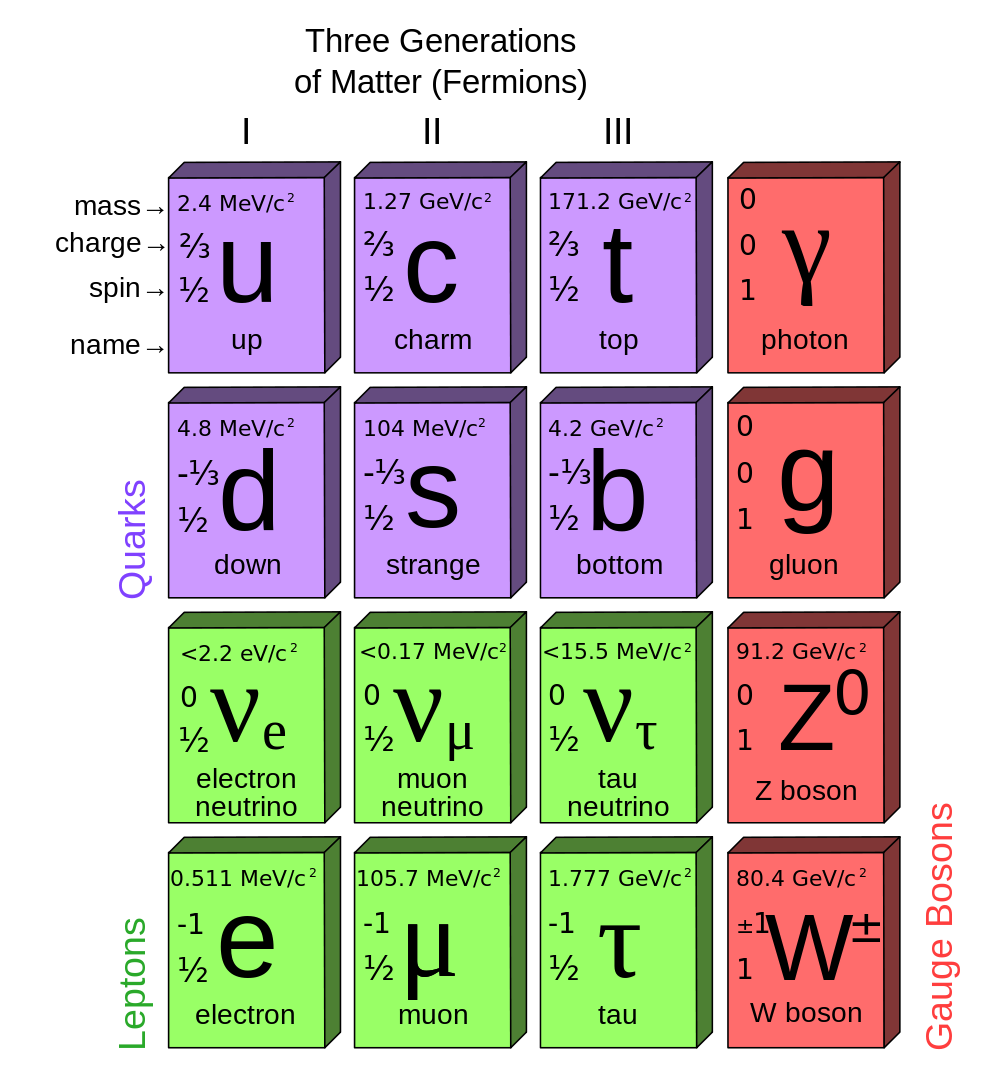
\includegraphics[width=.7\linewidth]{Introduction/figures/fundamentals.png}
\caption[Fundamental Particles of The Standard Model Before the LHC - FIND BETTER SOURCE]{The Fundamental Particles of the Standard Model and their Properties Before the LHC. Masses are listed in units of $eV/c^2$, a convenient unit for quantifying subatomic masses.}
\label{fig:fundamentals}
\end{center}
\end{figure}

Before the LHC was turned on, this (Fig~\ref{fig:fundamentals}) was the status of the observed particles and properties of the Standard Model. Absent from this picture is the Higgs boson. To understand the role of the Higgs boson and the importance of its discovery, we need to step back and motivate the Standard Model itself.

\subsection{The Story: The Status of the Standard Model Before the LHC}
\label{sec:SMpreLHC}

Trying to encapsulate the entire universe at once is undeniably intimidating. Fortunately, over centuries of development, physicists have established an arsenal of tools to make the task a bit more manageable. One of the most powerful techniques available is to locate and utilize a symmetry in the phenomenon to be considered; a planet should rotate around a star in the same fashion whether it's moving clockwise or counterclockwise. More than just identifying the symmetry to help simplify a problem, Noether's Theorem states if a system has a particular symmetry it inherently has an associated observed quantity. These examples are prolific, forming the basis of even introductory physics:

\begin{description}
\item[Conservation of Energy]
Time invariant Lagrangians\footnote{Lagrangians, referred to by $\Lagr$, are mathematical formulations which detail the dynamics of a given system.} conserve energy.
\item[Conservation of Momentum]
Translationally invariant Lagrangians conserve momentum.
\item[Conservation of Angular Momentum]
Rotationally invariant Lagrangians conserve angular momentum.
\end{description}

Symmetries themselves divide into two categories: global and local. Global symmetries apply to each point in the system equally, whereas local symmetries apply to individual points in the system. To picture the difference, imagine a grassy field where thousands of identical red balls have been placed in a grid. When you rotate all of the balls 10 degrees, this is a global transformation. If you rotate just one ball 10 degrees, this is a local transformation. In either case, the orientations of the balls will not appear to have changed, so the system has both a global and local symmetry.

The entire Standard Model can be described by only a few symmetries. Globally, the Standard Model obeys \textit{Poincar\'{e} symmetry}, which encapsulates all the symmetries we expect: translational (dynamics are invariant of location), rotational (dynamics unchanged by fixed rotation), time (dynamics will be identical regardless of when they start), and boosts (dynamics don't change if the whole system is moving at a uniform speed). Further, the Standard Model has three local symmetries which correspond to each of the three forces covered by the SM. Each of these local symmetries is called a {\it gauge symmetry} and has associated bosons called {\it gauge bosons} whose number is determined by the number of free parameters of the symmetry.

Electromagnetism, for example, has a gauge symmetry defined by U(1), the group associated with rotations about one axis. Since these rotations are only be defined by one angle, there should be just one gauge boson associated with electromagnetism. As explained in Sec.~\ref{sec:FundParticles}, the Standard Model has exactly that: the photon is this gauge boson. Indeed, gauge bosons are force carriers and vice versa. The weak force has a local symmetry of SU(2) and thus should have three gauge bosons\footnote{For brevity, the explanation for the number of bosons implied by SU(N) and the mathematics behind these groups are not provided, but detailed further in INSERT SU(N) REFERENCE}, which appear at first glance to match the $W^{\pm}$ and $Z$ bosons. The strong force has a local symmetry of SU(3) and has eight gauge bosons which match the eight gluons\footnote{Aside from a brief reprise dealing with hadronization in Sec.~\ref{sec:HadrCalo}, the strong force doesn't relate to the remainder of this thesis. Further information can be found at INSERT QCD REFERENCE}. Thus, we have our picture of fundamental fermions exchanging these gauge bosons to interact with one another.

However, mass has not yet been motivated. In fact, gauge bosons are mathematically required to be massless particles. Although the photon and the gluons are massless, why do the $W^{\pm}$ and $Z^{0}$ bosons have mass? The mass hierarchy of the fermions is also absent: if the top and up have otherwise identical properties, why is the top's mass over 75,000 times greater than the up? More problems arise: if matter and antimatter annihilate when they collide, why is there more matter than antimatter? And what about gravity? These are the deeper concerns of the Standard Model. Fortunately, there are answers that, if correct, could leave signatures we could find in particle accelerators.

\subsubsection{Searching for Professor Higgs' Boson}
\label{sec:findinghiggs}

Another common theme motivating the SM and physics beyond the SM is the idea of unification, all forces are simply different aspects of a single force. In 1961, Sheldon Glashow observed that electromagnetism and the weak force could be unified in the electroweak interaction~\cite{Glashow:1961}. In short, the unified U(1)$\times$SU(2) electroweak theory has one boson associated with U(1) ($B^{0}$) and three bosons associated with SU(2) (one neutrally charged $W^{0}$ and two charged bosons, $W^{+}$ and $W^{-}$). This symmetry is then broken such that the photon and $Z^{0}$ are mixtures of both the $B^{0}$ and $W^{0}$. Breaking a gauge invariance can introduce mass terms for the gauge bosons, so while the photon will be massless, the $W^{\pm}$ and $Z^{0}$ will be massive. This does provide the desired result, but it shifts the burden; there ought to be an explanation why this symmetry is broken. Shortly after this unification was proposed, a framework was proposed which explains how a gauge symmetry could be spontaneously broken instead of explicitly broken~\cite{Anderson:1963pc,Higgs:1964,Englert:1964,Higgs:1964-2,Guralnik:1964}: the \textit{Higgs Mechanism}. 

The Higgs mechanism details that there is a field that fills all of space and interacts with the particles of the Standard Model. How this gives a broken symmetry is best illustrated by looking at the associated potential. At high energies, we can picture the potential to be a symmetric valley centered around a point. In that case, the lowest energy state is stable and symmetric: if we imagine a ball rolling in such a structure, it would always come to the lowest point and the symmetry is preserved. But, as the universe cooled, the Higgs potential changed to what is seen in Fig.~\ref{fig:HiggsPotential}, commonly referred to as the ``Mexican-hat" or ``champagne bottle potential". As the ball started at the top of the bulge, it would fall to a lower energy state in the circular valley. Clearly, the symmetry that was preserved in the early universe would then be broken.

\begin{figure}[hbt]
\begin{center}
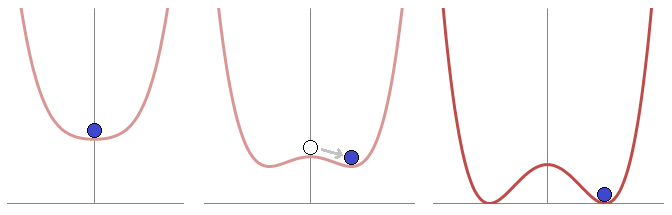
\includegraphics[width=.7\linewidth]{Introduction/figures/SpontaneousSymmetryBreaking.png}
\caption[The Higgs Mechanism - FROM WIKIPEDIA]{The Higgs Potential is a quartic potential with a negative quadratic term. This change in sign gives a ring of energetically favorable values, which provide the spontaneous symmetry breaking required by the Standard Model.}
\label{fig:HiggsPotential}
\end{center}
\end{figure}

This mechanism, along with the other fundamental forces and particles, was summarized into the Standard Model by Weinberg and Salam~\cite{Weinberg:1967,Salam:1968}. In doing so, we have a natural explanation for the massless photon and massive $W^{\pm}$ and $Z^{0}$ that we require. The massive $Z^{0}$ in particular had only been predicted when the Standard Model was finalized in the late 1960s, but in the coming decades it was observed indirectly in the 1970s~\cite{} and then directly in the 1980s~\cite{}. On top of making the $W^{\pm}$ and $Z^{0}$ massive, by breaking the Electroweak symmetry fermions acquire a mass proportional to how strongly they couple to the Higgs field. This explains why the top and the up have such greatly differing masses.

Crucially, the completion of the Standard Model with the Higgs mechanism from an experimental perspective is to confirm that the Higgs field exists and does generate the masses as described. The final prediction of the Standard Model is that there should be excitations of the Higgs field which manifest as the \textit{Higgs boson}, commonly shortened to just ``the Higgs", which is an uncharged zero-spin particle. The strength that bosons and fermions couple to the Higgs field is only determined by the mass of the Higgs boson, so the only unknown in the SM before the LHC was what this mass is.

Before the LHC, all attempts to find the Higgs boson had been elusive. Theoretically, $m_{H}\lesssim1$~TeV otherwise there would be large instabilities in the universe that would have already been observed~\cite{}. A lower bound on the Higgs mass was set at LEP, an electron-positron collider, where $m_{H}>114.4$~GeV~\cite{Barate:2003sz} at the 95\% confidence level. From measuring properties of the SM to higher and higher precision, the Higgs mass was expected to be found in the mass range $m_{H}\lesssim185GeV$. Since the exact Higgs mass was not known and these excitations should be extraordinarily rare, the best chance to find the predicted Higgs would be a general purpose detector at a particle accelerator that scans a wide range of energies with a very high throughput. The Tevatron is such a collider and its general detectors, D0 and CDF, further excluded the Higgs from having a mass between $160<m_{H}<170$~GeV~\cite{Aaltonen:2010yv}, leading to the status showing in Fig.~\ref{fig:HiggsExclusionPreLHC} In Sec.~\ref{sec:expt}, we argue that the CMS detector at the LHC is ideal for extending this search.

\begin{figure}[hbt]
\begin{center}
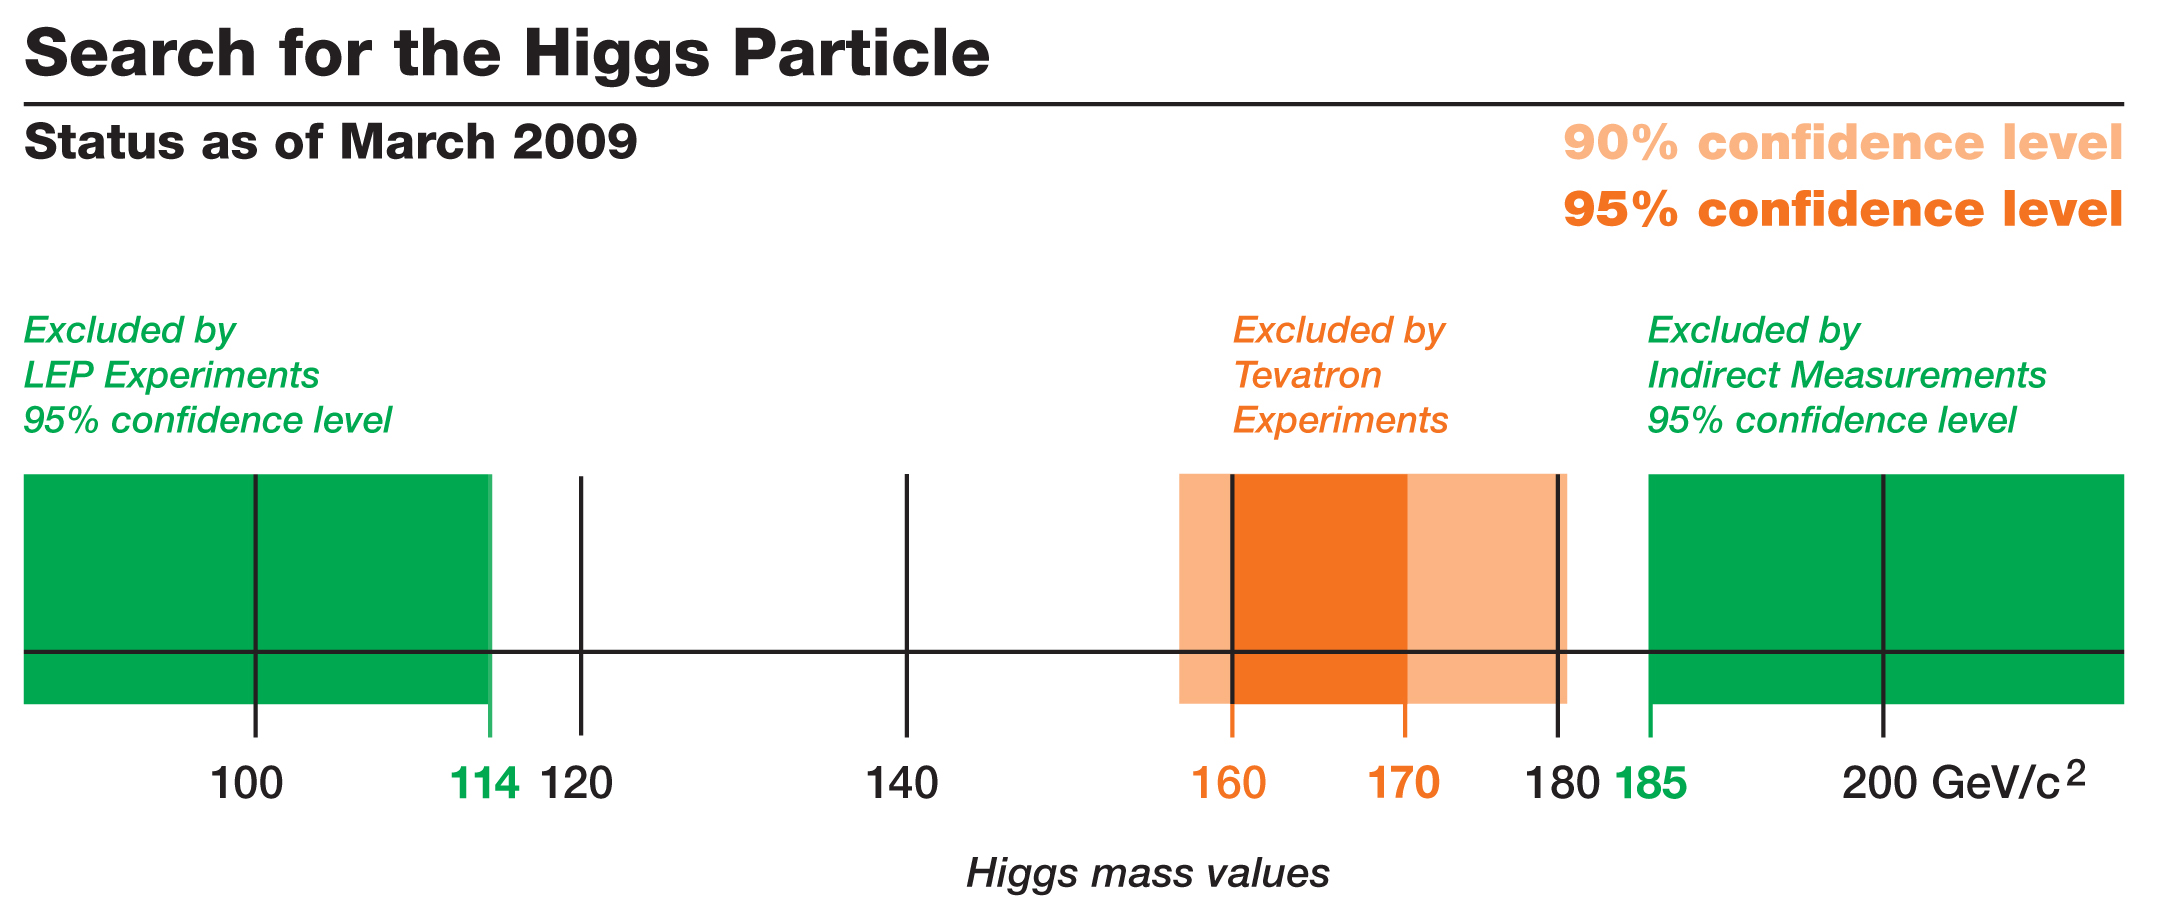
\includegraphics[width=.7\linewidth]{Introduction/figures/HiggsExclusions_09.jpg}
\caption[Higgs Mass Limits Before the LHC]{Before the LHC, the Higgs Boson's mass was excluded to 95\% confidence in the ranges $m_{H}<114.4$~GeV, $160<m_{H}<170$~GeV, and $m_{H}>185$~GeV.}
\label{fig:HiggsExclusionPreLHC}
\end{center}
\end{figure}

\subsubsection{Expecting the Unexpected}
\label{sec:findingBSM}

Adding the Higgs Boson to our cast of fundamental particles completes the Standard Model, but there are still remaining difficulties:

\begin{description}
\item[Matter v Antimatter] \hfill \\
Matter and antimatter annihilate when they interact, yet the visible universe is largely made of matter. The current theoretical explanation for this asymmetry is that there are particles and decays that would have a preference for matter over antimatter~\cite{}. Although some of this asymmetry has been predicted and observed, neither are sufficient to account for the relative lack of antimatter.
\item[Gravity] \hfill \\
Gravity is notoriously absent from the SM. Its inclusion is extraordinarily difficult. Gravity is many orders of magnitude weaker than any of the other three forces and must appear like General Relativity at large distances, but currently quantum models of gravity break down at very small distances.
\item[Neutrino Masses] \hfill \\
In the SM, neutrinos are not predicted to have mass, yet they have been observed to oscillate between different generations~\cite{}. In order to account for these oscillations, the neutrinos are required to have different masses and thus must be massive.
\item[Dark Matter and Dark Energy] \hfill \\
Current estimates of the universe say that only 4\% of all mass-energy is made of the particles in the Standard Model. The remaining 96\% is made up of Dark Matter (23\%) which seems to only interact gravitationally and Dark Energy (73\%) which is responsible for the acceleration of the expansion of the universe.
\end{description}

These questions lead to models that are considered Beyond the Standard Model (BSM) physics. There are two main veins of BSM physics, Supersymmetry (SUSY) and Extra Dimensions. As discussed already, symmetry is a very powerful tool in theoretical physics. SUSY takes the symmetries available under the SM and adds one additional symmetry which predicts new supersymmetric partners for every particle in the SM. For example, every fermion will have a supersymmetric bosonic partner, e.g. the selectron to the electron or the sbottom to the bottom. These partners could provide answers for some or all of the unresolved questions in the SM. Extra dimensions posits that beyond the four traditional dimensions, three spatial and one time, there are additional dimensions which are not readily observed. Additional particles and properties can be hidden in excitations of these extra dimensions which could also explain these unresolved questions.

These additional particles and properties influence searches at the LHC aside from direct observation. First and foremost, nearly all BSM models would require not just one but multiple Higgs bosons, any or all of which could be probed at the LHC. Thus, even though the Higgs of the SM is most likely to be found in the mass range $<m_{H}<$, the search should be extended to look for other resonances which may be Higgs-like that would give credence to BSM physics. Furthermore, each of these particles could have different properties than what we expect in the SM Higgs mechanism. Many theorized explanations of gravity imply the existence of another boson called the graviton. Such a particle would have spin-2 instead of the spin-0 presumed in the SM Higgs, so it is also important to probe the spin of any new particle.

Some new physics comes from looking at high precision measurements which predicate the discovery of undiscovered fundamental particles, as was predicted with the $Z^{0}$. For example to achieve the matter/antimatter asymmetry, there need to be particles that violate CP-symmetry, where a system's dynamics are identical if all matter is replaced with antimatter (and vice versa) and the spatial coordinates are inverted. Given that the CP-symmetry needed to explain the matter/antimatter asymmetry has not yet been observed, the hope is that new particles would break this symmetry. Even if no other particles aside from a Higgs candidate are found, the SM Higgs is predicted to preserve this symmetry (\textit{CP-even}) and any deviation in the properties from the expected could prove invaluable towards future research into the field of particle physics.

\section{Summary}
\label{sec:intro_summary}

As previously mentioned, we now know that there is a Higgs boson, but it is insightful in retrospect to walk through the discovery chronologically to understand the process and appreciate its significance. In Sec.~\ref{sec:expt}, the LHC will be expounded, particularly the CMS experiment and how it was designed to look for a Higgs boson or other new physics. In Sec.~\ref{sec:pheno}, one possible signature of the Higgs will be investigated, including why it is considered the ``golden" channel and how it has been crucial to the discovery of the boson and its properties. In Sec.~\ref{sec:results}, the observed properties will be detailed and how well they match up with what we expect in the Standard Model. Lastly, in Sec.~\ref{sec:conclusions}, the effects of these results will be summarized and what they mean for future measurements.